\documentclass[aspectratio=169]{beamer}

% ---------- ENCODING & FONTS ----------
\usepackage[utf8]{inputenc}
\usepackage[T1]{fontenc}

% ---------- THEME & LOOK ----------
\usetheme{Madrid}
\usecolortheme{seahorse}
\usefonttheme{professionalfonts}
\setbeamertemplate{navigation symbols}{}
\setbeamercovered{transparent}
\setbeamertemplate{itemize items}[circle]
\setbeamertemplate{enumerate items}[default]
\setlength{\parskip}{0.25em}

% ---------- COLORS ----------
% Beamer already loads xcolor, so we just define our colors
\definecolor{accent}{RGB}{0,92,184}
\definecolor{soft}{RGB}{233,244,255}
\definecolor{lightred}{RGB}{245,210,210}
\setbeamercolor{structure}{fg=accent}
\setbeamercolor{title}{fg=white,bg=accent}
\setbeamercolor{frametitle}{fg=accent}
\setbeamercolor{block title}{bg=accent!12,fg=accent}
\setbeamercolor{block body}{bg=soft}

% ---------- PACKAGES ----------
\usepackage{booktabs}
\usepackage{amsmath, amssymb}
\usepackage{array}
\usepackage{multirow}
\usepackage{hyperref}
\hypersetup{colorlinks=true,linkcolor=accent,urlcolor=accent}

% ---------- SAFE TRANSITION FALLBACK ----------
\makeatletter
\@ifundefined{transfade}{\newcommand{\transfade}[1][]{}}{}
\makeatother

% ---------- PLACEHOLDER BOX FOR FIGURES ----------
\newcommand{\placeholderbox}[2][0.82\linewidth]{%
  \begin{center}
    \fbox{\begin{minipage}[c][0.46\textheight][c]{#1}
      \centering \vspace{0.3em}
      \textbf{#2}\\[0.6em]
      \emph{Insert figure/diagram here later.}
    \end{minipage}}
  \end{center}
}
% ---------- TITLE ----------
\title{\textbf{Economic Growth, the Financial System, and Business Cycles  \vspace{.5cm}\\  }}
\subtitle{ {\large ECON 101 - Macroeconomics}}
%\institute{UNBC}
\author{Muhebullah Karimzada}
\date{Winter 2026}


\begin{document}

% ============================================================
% TITLE
% ============================================================
\begin{frame}[plain]
  \titlepage
\end{frame}

% ============================================================
\begin{frame}{Chapter Outline}
\transfade
\begin{itemize}[<+->]
  \item \textbf{6.1} Long-Run Economic Growth
  \item \textbf{6.2} Saving, Investment, and the Financial System
  \item \textbf{6.3} The Business Cycle
\end{itemize}
\end{frame}

% ============================================================
\section{6.1 Long-Run Economic Growth}
% ============================================================

\begin{frame}{6.1 Learning Objective}
\transfade
\begin{block}{Goal}
Explain how long-run economic growth is measured and what determines it.
\end{block}
\begin{itemize}[<+->]
  \item \textbf{Long-run economic growth:} the process by which rising \alert{productivity} increases the \textbf{average standard of living}.
  \item This is different from short-run fluctuations (\textbf{business cycles}):
  \begin{itemize}[<+->]
    \item \textbf{Expansion:} real GDP rising.
    \item \textbf{Recession:} real GDP falling.
  \end{itemize}
  \item The most common measure of the standard of living is:
  \begin{itemize}[<+->]
    \item \textbf{Real GDP per capita} = real GDP divided by population.
  \end{itemize}
\end{itemize}
\end{frame}

\begin{frame}{Real GDP per Capita: A Key Indicator}
\transfade
\begin{itemize}[<+->]
  \item \textbf{Real GDP per capita} tells us:
  \begin{itemize}[<+->]
    \item How much goods and services, on average, each person can consume.
    \item Adjusted for changes in the price level (\textbf{real}, not nominal).
  \end{itemize}
  \item It does not capture everything about well-being, but:
  \begin{itemize}[<+->]
    \item Countries with higher real GDP per capita typically have better:
    \begin{itemize}[<+->]
      \item health, education, housing, and infrastructure.
    \end{itemize}
  \end{itemize}
\end{itemize}
\end{frame}

\begin{frame}{Figure 6.1 -- Real GDP per Capita, 1961--2021}
\centering
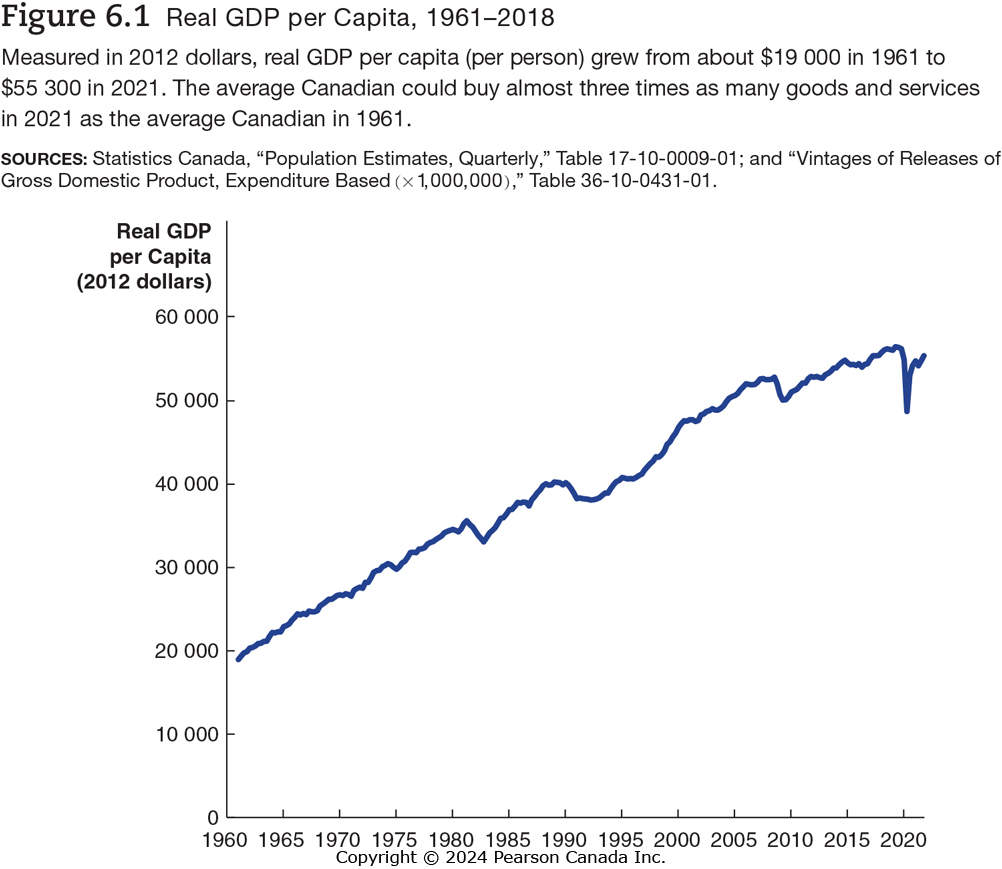
\includegraphics[width=0.61\linewidth]{Fig06-001}.
\end{frame}

\begin{frame}{Interpretation of Figure 6.1}
\transfade
\begin{itemize}[<+->]
  \item Measured in 2012 dollars, real GDP per capita in Canada has risen more than \textbf{three-fold} since 1961.
  \item Interpretation:
  \begin{itemize}[<+->]
    \item The average Canadian in 2021 can buy almost \alert{three times as many} goods and services as the average Canadian in 1961.
  \end{itemize}
  \item This long-run rise is what we mean by \textbf{economic growth}.
  \item Short-run recessions are bumps around this upward trend.
\end{itemize}
\end{frame}

% ------------------------------------------------------------
% Growth Rates & Rule of 70
% ------------------------------------------------------------

\begin{frame}{Calculating Growth Rates}
\transfade
\begin{itemize}[<+->]
  \item Growth rate of an economic variable (e.g., real GDP) from year \(t-1\) to year \(t\):
  \[
    \text{Growth rate}_t =
    \frac{\text{Value}_t - \text{Value}_{t-1}}{\text{Value}_{t-1}} \times 100.
  \]
  \item For a few years, we can compute growth each year and then take the average.
  \item Example:
  \begin{itemize}[<+->]
    \item Real GDP per capita grows by 2\%, 3\%, and 1\% over three years.
    \item Average annual growth \(\approx (2 + 3 + 1)/3 = 2\%\).
  \end{itemize}
\end{itemize}
\end{frame}

\begin{frame}{Growth Rates over Longer Periods}
\transfade
\begin{itemize}[<+->]
  \item Over longer periods, we use \textbf{compound growth}.
  \item Suppose:
  \begin{itemize}[<+->]
    \item Previous real GDP = \(Y_0\),
    \item Current real GDP = \(Y_t\),
    \item Annual growth rate = \(g\),
    \item Number of years between = \(t\).
  \end{itemize}
  \item Then:
  \[
    Y_0 (1 + g)^t = Y_t.
  \]
  \item Solving for \(g\) gives the average annual growth rate over the period.
\end{itemize}
\end{frame}

\begin{frame}{The Rule of 70}
\transfade
\begin{itemize}[<+->]
  \item A handy shortcut: the \textbf{Rule of 70}.
  \item If a variable grows at rate \(g\%\) per year, the number of years it takes to \textbf{double} is approximately:
  \[
    \text{Years to double} \approx \frac{70}{g}.
  \]
  \item Example:
  \begin{itemize}[<+->]
    \item If real GDP per capita grows at 5\% per year:
    \item Years to double \(\approx 70 / 5 = 14\) years.
  \end{itemize}
  \item This shows how even small differences in growth rates matter a lot over time.
\end{itemize}
\end{frame}

\begin{frame}{Rule of 70: Classroom Example}
\transfade
\begin{itemize}[<+->]
  \item If Country A grows at 2\% per year:
  \begin{itemize}[<+->]
    \item It takes about \(70/2 = 35\) years to double income per person.
  \end{itemize}
  \item If Country B grows at 4\% per year:
  \begin{itemize}[<+->]
    \item It takes about \(70/4 = 17.5\) years to double.
  \end{itemize}
  \item After a few decades, Country B will be much richer than Country A, even though the growth rate difference seems small.
\end{itemize}
\end{frame}

% ------------------------------------------------------------
% What Determines Long-Run Growth?
% ------------------------------------------------------------

\begin{frame}{What Determines Long-Run Growth?}
\transfade
\begin{itemize}[<+->]
  \item Long-run increases in real GDP per capita depend on increases in \textbf{labour productivity}:
  \[
    \text{Labour productivity} =
    \frac{\text{Real GDP}}{\text{Number of workers or hours worked}}.
  \]
  \item The average Canadian today consumes more because:
  \begin{itemize}[<+->]
    \item the average Canadian \textbf{produces} much more per hour than in 1961.
  \end{itemize}
  \item So, what makes workers more productive?
\end{itemize}
\end{frame}

\begin{frame}{Factors Affecting Labour Productivity Growth}
\transfade
\begin{itemize}[<+->]
  \item Two key factors:
  \begin{itemize}[<+->]
    \item \textbf{Increases in capital per hour worked}
    \item \textbf{Technological change}
  \end{itemize}
\end{itemize}
\end{frame}

\begin{frame}{Capital per Hour Worked}
\transfade
\begin{itemize}[<+->]
  \item \textbf{Capital:} durable manufactured goods used to produce other goods and services.
  \begin{itemize}[<+->]
    \item Machines, computers, tools, buildings, vehicles.
  \end{itemize}
  \item The more capital each worker has, the more they can produce per hour.
  \item Also important: \textbf{human capital}:
  \begin{itemize}[<+->]
    \item The accumulated \alert{knowledge and skills} workers possess (education, training, experience).
  \end{itemize}
  \item Example:
  \begin{itemize}[<+->]
    \item A worker with a modern computer and software is usually more productive than one with only pen and paper.
  \end{itemize}
\end{itemize}
\end{frame}

\begin{frame}{Technological Change}
\transfade
\begin{itemize}[<+->]
  \item \textbf{Technological change:} improvements in methods of combining inputs into outputs.
  \item Examples:
  \begin{itemize}[<+->]
    \item New production processes,
    \item Better management techniques,
    \item New products (e.g., smartphones, advanced medical devices).
  \end{itemize}
  \item With better technology, workers can produce more \textbf{with the same amount} of capital and labour.
  \item \textbf{Entrepreneurs} play a critical role:
  \begin{itemize}[<+->]
    \item They pioneer new ways to bring together labour, capital, and ideas.
  \end{itemize}
\end{itemize}
\end{frame}

% ------------------------------------------------------------
% Potential GDP & Output Gap
% ------------------------------------------------------------

\begin{frame}{Potential GDP}
\transfade
\begin{itemize}[<+->]
  \item \textbf{Potential GDP:} level of real GDP attained when all firms are producing at \textbf{capacity}.
  \item Capacity here means:
  \begin{itemize}[<+->]
    \item “Normal” hours,
    \item “Normal” sized workforce,
    \item No special overtime or emergency use of capital.
  \end{itemize}
  \item Potential GDP increases when:
  \begin{itemize}[<+->]
    \item labour force grows,
    \item more factories are built,
    \item more equipment is installed,
    \item technological change occurs.
  \end{itemize}
\end{itemize}
\end{frame}

\begin{frame}{Figure 6.2 -- The Output Gap }
\centering
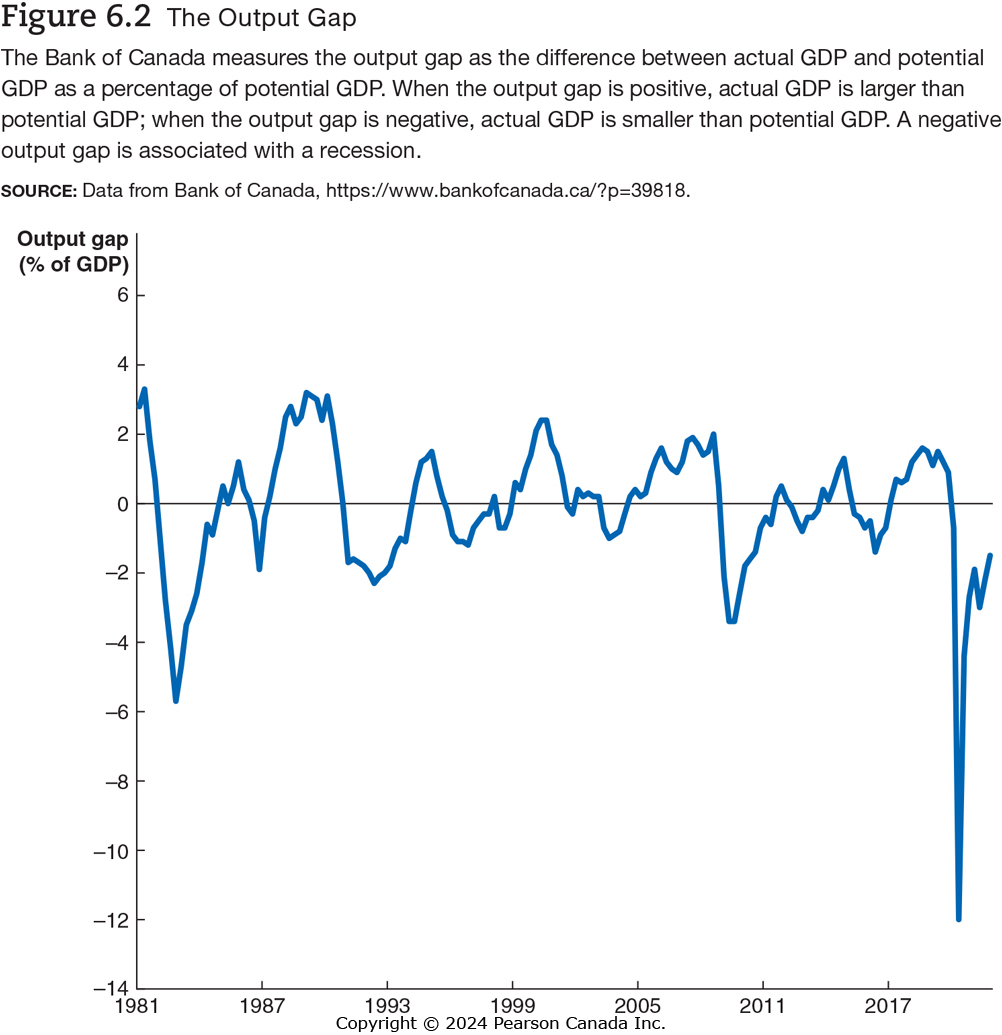
\includegraphics[width=0.61\linewidth]{Fig06-002}.
\end{frame}

\begin{frame}{The Output Gap}
\transfade
\begin{itemize}[<+->]
  \item \textbf{Output gap:} difference between actual GDP and potential GDP.
  \item When the output gap is \textbf{positive}:
  \begin{itemize}[<+->]
    \item actual GDP is above potential,
    \item the economy is using resources in an \alert{unsustainable} way (very low unemployment, high capacity usage).
  \end{itemize}
  \item When the output gap is \textbf{negative}:
  \begin{itemize}[<+->]
    \item actual GDP is below potential,
    \item resources (labour and capital) are \alert{underutilized}.
  \end{itemize}
  \item The Bank of Canada pays close attention to the output gap when setting interest rates.
\end{itemize}
\end{frame}

% ============================================================
\section{6.2 Saving, Investment, and the Financial System}
% ============================================================

\begin{frame}{6.2 Learning Objective}
\transfade
\begin{block}{Goal}
Explain how the financial system links saving and investment and why that matters for growth.
\end{block}
\begin{itemize}[<+->]
  \item Long-run growth requires:
  \begin{itemize}[<+->]
    \item more capital per worker, and
    \item ongoing technological improvements.
  \end{itemize}
  \item Both require \textbf{investment}.
  \item Investment is financed by \textbf{saving}, and the financial system connects savers and borrowers.
\end{itemize}
\end{frame}

% ------------------------------------------------------------
% Overview of the Financial System
% ------------------------------------------------------------

\begin{frame}{An Overview of the Financial System}
\transfade
\begin{itemize}[<+->]
  \item \textbf{Financial markets:} markets where financial securities are bought and sold.
  \begin{itemize}[<+->]
    \item Examples: stock markets, bond markets.
  \end{itemize}
  \item \textbf{Financial security:} document (often electronic) stating terms under which funds pass from buyer to seller.
  \item \textbf{Stock:} financial security representing partial ownership of a firm.
  \item \textbf{Bond:} financial security promising to repay a fixed amount of funds.
  \begin{itemize}[<+->]
    \item In effect, a bond is a \textbf{loan} from households to firms or governments.
  \end{itemize}
\end{itemize}
\end{frame}

\begin{frame}{Financial Intermediaries}
\transfade
\begin{itemize}[<+->]
  \item \textbf{Financial intermediaries:} firms that borrow funds from savers and lend them to borrowers.
  \item Examples:
  \begin{itemize}[<+->]
    \item banks,
    \item mutual funds,
    \item pension funds,
    \item insurance companies.
  \end{itemize}
  \item Example:
  \begin{itemize}[<+->]
    \item Mutual funds sell shares to savers,
    \item then use the funds to buy a diversified portfolio of stocks and bonds.
  \end{itemize}
\end{itemize}
\end{frame}

\begin{frame}{Three Key Services of the Financial System}
\transfade
\begin{itemize}[<+->]
  \item The financial system provides three key services:
  \begin{enumerate}[<+->]
    \item \textbf{Risk-sharing}
    \item \textbf{Liquidity}
    \item \textbf{Information}
  \end{enumerate}
\end{itemize}
\end{frame}

\begin{frame}{Risk-Sharing}
\transfade
\begin{itemize}[<+->]
  \item \textbf{Risk-sharing:}
  \begin{itemize}[<+->]
    \item Savers can spread their money over many different assets.
    \item This reduces risk while maintaining a high expected return.
  \end{itemize}
  \item Example:
  \begin{itemize}[<+->]
    \item Buying shares in a mutual fund instead of investing all savings in one firm.
  \end{itemize}
\end{itemize}
\end{frame}

\begin{frame}{Liquidity}
\transfade
\begin{itemize}[<+->]
  \item \textbf{Liquidity:} the ease with which a financial asset can be converted into cash.
  \item The financial system provides liquid assets:
  \begin{itemize}[<+->]
    \item bank accounts,
    \item money market mutual funds,
    \item actively traded bonds and stocks.
  \end{itemize}
  \item This allows savers to commit funds while still being able to access cash when needed.
\end{itemize}
\end{frame}

\begin{frame}{Information}
\transfade
\begin{itemize}[<+->]
  \item \textbf{Information:}
  \begin{itemize}[<+->]
    \item Prices of financial securities reflect the expectations of many investors about future returns.
  \end{itemize}
  \item The financial system aggregates information about:
  \begin{itemize}[<+->]
    \item firm profitability,
    \item riskiness of projects,
    \item macroeconomic conditions.
  \end{itemize}
  \item This guides funds toward the most promising investment opportunities.
\end{itemize}
\end{frame}

% ------------------------------------------------------------
% Saving and Investment: Macroeconomic Identity
% ------------------------------------------------------------

\begin{frame}{The Macroeconomics of Saving and Investment}
\transfade
\begin{itemize}[<+->]
  \item Start from the national income identity:
  \[
    Y = C + I + G + NX.
  \]
  \item For simplicity, assume a \textbf{closed economy} (no exports or imports), so:
  \[
    Y = C + I + G.
  \]
  \item Rearranging to solve for investment:
  \[
    I = Y - C - G.
  \]
  \item Investment equals total income not used for consumption or government purchases.
\end{itemize}
\end{frame}

\begin{frame}{Private Saving and Public Saving}
\transfade
\begin{itemize}[<+->]
  \item \textbf{Private saving} (\(S_{\text{private}}\)):
  \begin{itemize}[<+->]
    \item Households receive income from factors of production (\(Y\)) and transfers (\(\text{TR}\)).
    \item They pay taxes (\(T\)) and consume (\(C\)).
  \end{itemize}
  \item So:
  \[
    S_{\text{private}} = Y + \text{TR} - C - T.
  \]
  \item \textbf{Public saving} (\(S_{\text{public}}\)):
  \begin{itemize}[<+->]
    \item The government receives tax revenue (\(T\)),
    \item and spends on purchases (\(G\)) and transfers (\(\text{TR}\)).
  \end{itemize}
  \item So:
  \[
    S_{\text{public}} = T - G - \text{TR}.
  \]
\end{itemize}
\end{frame}

\begin{frame}{Total Saving and Investment}
\transfade
\begin{itemize}[<+->]
  \item \textbf{Total saving} is:
  \[
    S = S_{\text{private}} + S_{\text{public}}.
  \]
  \item Substitute the formulas:
  \begin{align*}
    S &= (Y + \text{TR} - C - T) + (T - G - \text{TR}) \\
      &= Y - C - G.
  \end{align*}
  \item But from earlier:
  \[
    I = Y - C - G.
  \]
  \item Therefore:
  \[
    S = I.
  \]
  \item In a closed economy, \textbf{saving equals investment}.
\end{itemize}
\end{frame}

\begin{frame}{Budget Balance and Crowding Out}
\transfade
\begin{itemize}[<+->]
  \item If \(S_{\text{public}} = 0\):
  \begin{itemize}[<+->]
    \item Government has a \textbf{balanced budget}.
  \end{itemize}
  \item If \(S_{\text{public}} < 0\):
  \begin{itemize}[<+->]
    \item Government runs a \textbf{budget deficit}.
    \item It must borrow (sell bonds), reducing funds available for private investment.
  \end{itemize}
  \item If \(S_{\text{public}} > 0\):
  \begin{itemize}[<+->]
    \item Government runs a \textbf{budget surplus}.
    \item It contributes to national saving.
  \end{itemize}
  \item When deficits reduce investment, we call this \textbf{crowding out}.
\end{itemize}
\end{frame}

% ------------------------------------------------------------
% Market for Loanable Funds
% ------------------------------------------------------------

\begin{frame}{The Market for Loanable Funds}
\transfade
\begin{itemize}[<+->]
  \item We can think of all financial markets together as one \textbf{market for loanable funds}.
  \item \textbf{Borrowers:} firms that want to invest in capital (and the government when it runs deficits).
  \item \textbf{Lenders:} households that save and lend funds, and sometimes foreign investors.
  \item The \textbf{real interest rate} is the price that equates saving and investment.
\end{itemize}
\end{frame}

\begin{frame}{Figure 6.3 -- The Market for Loanable Funds}
\centering
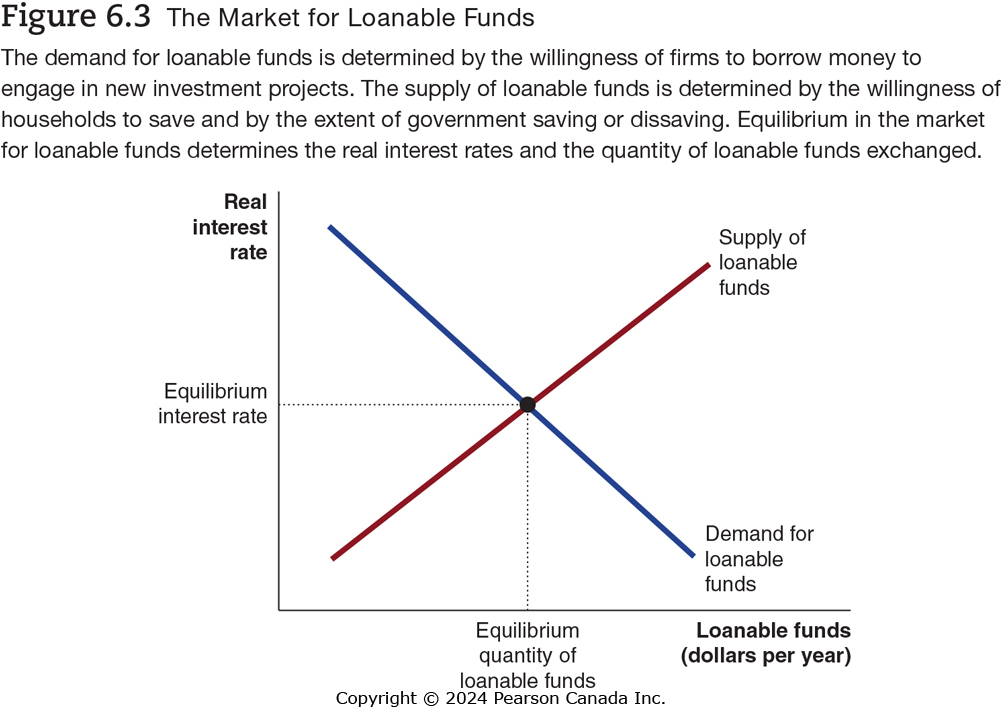
\includegraphics[width=0.67\linewidth]{Fig06-003}.
\end{frame}

\begin{frame}{Supply and Demand for Loanable Funds}
\transfade
\begin{itemize}[<+->]
  \item \textbf{Demand for loanable funds:}
  \begin{itemize}[<+->]
    \item Firms borrow more when the real interest rate is lower,
    \item because more investment projects are profitable.
  \end{itemize}
  \item \textbf{Supply of loanable funds:}
  \begin{itemize}[<+->]
    \item Households save more when the real interest rate is higher,
    \item because the reward for postponing consumption is greater.
  \end{itemize}
  \item Government saving (or dissaving) also affects supply.
\end{itemize}
\end{frame}

\begin{frame}{Figure 6.4 -- Increase in Demand for Loanable Funds }
\centering
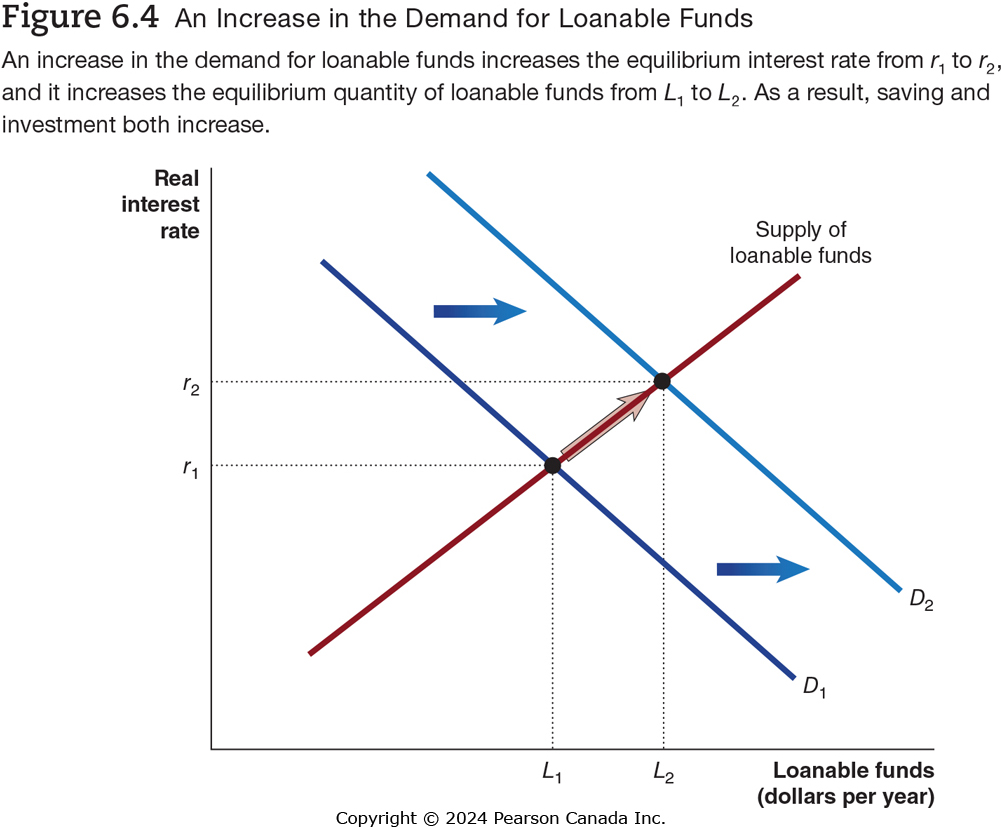
\includegraphics[width=0.61\linewidth]{Fig06-004}.
\end{frame}

\begin{frame}{Increase in Demand for Loanable Funds}
\transfade
\begin{itemize}[<+->]
  \item Suppose technological change makes investment more profitable.
  \item Firms want to borrow more at each interest rate.
  \item \textbf{Result:}
  \begin{itemize}[<+->]
    \item Demand for loanable funds shifts right.
    \item Equilibrium real interest rate rises.
    \item Equilibrium quantity of loanable funds (investment) rises.
  \end{itemize}
\end{itemize}
\end{frame}

\begin{frame}{Figure 6.5 -- Increase in Supply of Loanable Funds}
\centering
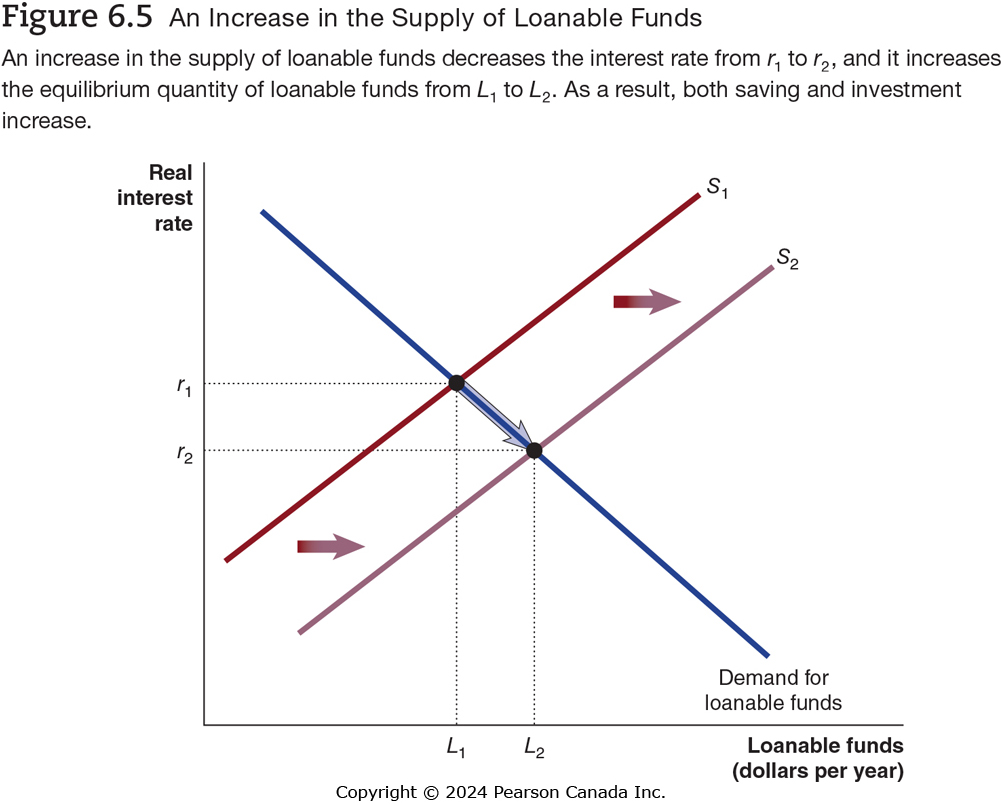
\includegraphics[width=0.61\linewidth]{Fig06-005}.
\end{frame}

\begin{frame}{Increase in Supply of Loanable Funds}
\transfade
\begin{itemize}[<+->]
  \item Suppose households become more patient or more concerned about retirement, and decide to save more at every interest rate.
  \item \textbf{Result:}
  \begin{itemize}[<+->]
    \item Supply of loanable funds shifts right.
    \item Equilibrium real interest rate falls.
    \item Equilibrium quantity of loanable funds (investment) rises.
  \end{itemize}
\end{itemize}
\end{frame}

\begin{frame}{Figure 6.6 -- Effect of a Budget Deficit }
\centering
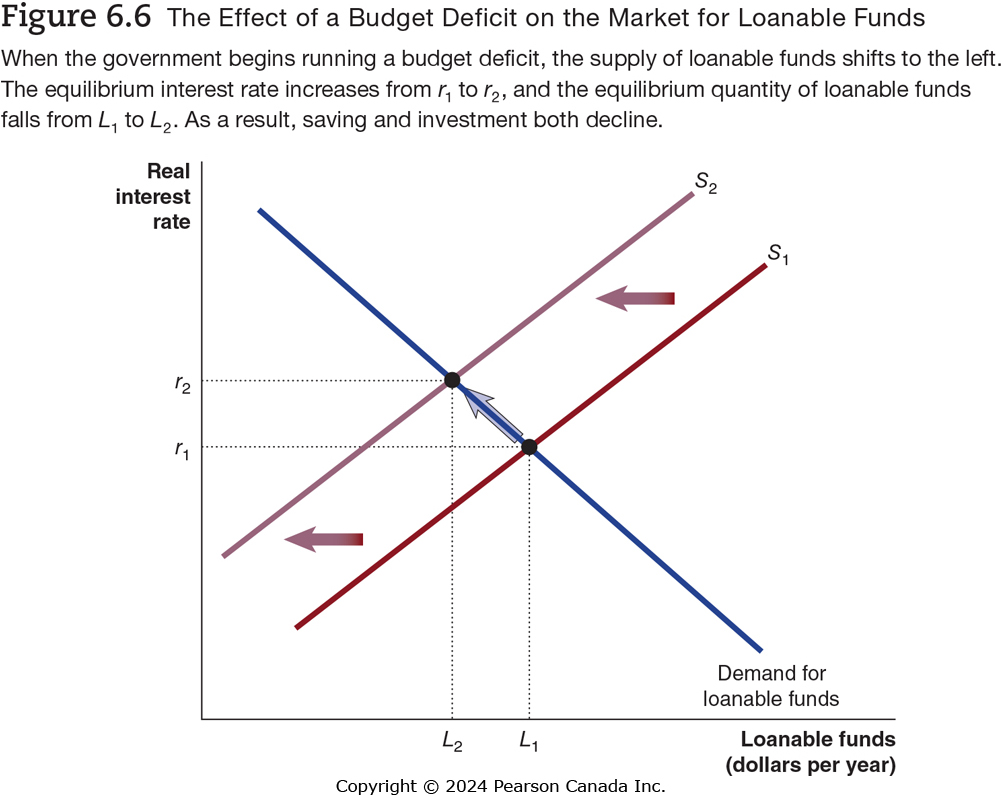
\includegraphics[width=0.61\linewidth]{Fig06-006}.
\end{frame}

\begin{frame}{Budget Deficits and Crowding Out}
\transfade
\begin{itemize}[<+->]
  \item When government runs a \textbf{budget deficit}, it must borrow funds.
  \item This reduces the funds available for private borrowers.
  \item In the loanable funds market:
  \begin{itemize}[<+->]
    \item Supply of loanable funds shifts left.
    \item Equilibrium real interest rate rises.
    \item Equilibrium quantity of funds to firms falls.
  \end{itemize}
  \item This reduction in private investment due to government borrowing is \textbf{crowding out}.
\end{itemize}
\end{frame}

\begin{frame}{How Important Is Crowding Out?}
\transfade
\begin{itemize}[<+->]
  \item In practice, the effect of deficits on interest rates is often \textbf{small}.
  \item Why?
  \begin{itemize}[<+->]
    \item Interest rates are influenced by \textbf{global saving}.
    \item Even several billion dollars of extra borrowing may be small relative to the world market.
  \end{itemize}
  \item Small does not mean zero:
  \begin{itemize}[<+->]
    \item Higher public debt may require higher taxes later.
    \item This can depress long-run growth.
  \end{itemize}
\end{itemize}
\end{frame}

% ============================================================
\section{6.3 The Business Cycle}
% ============================================================

\begin{frame}{6.3 Learning Objective}
\transfade
\begin{block}{Goal}
Explain what happens during the business cycle and how it affects inflation and unemployment.
\end{block}
\begin{itemize}[<+->]
  \item Real GDP per capita has risen about threefold since 1961.
  \item But it did not rise \textbf{smoothly}—there were periods of recession and expansion.
\end{itemize}
\end{frame}

\begin{frame}{Figure 6.7 -- The Business Cycle (Idealized)}
\centering
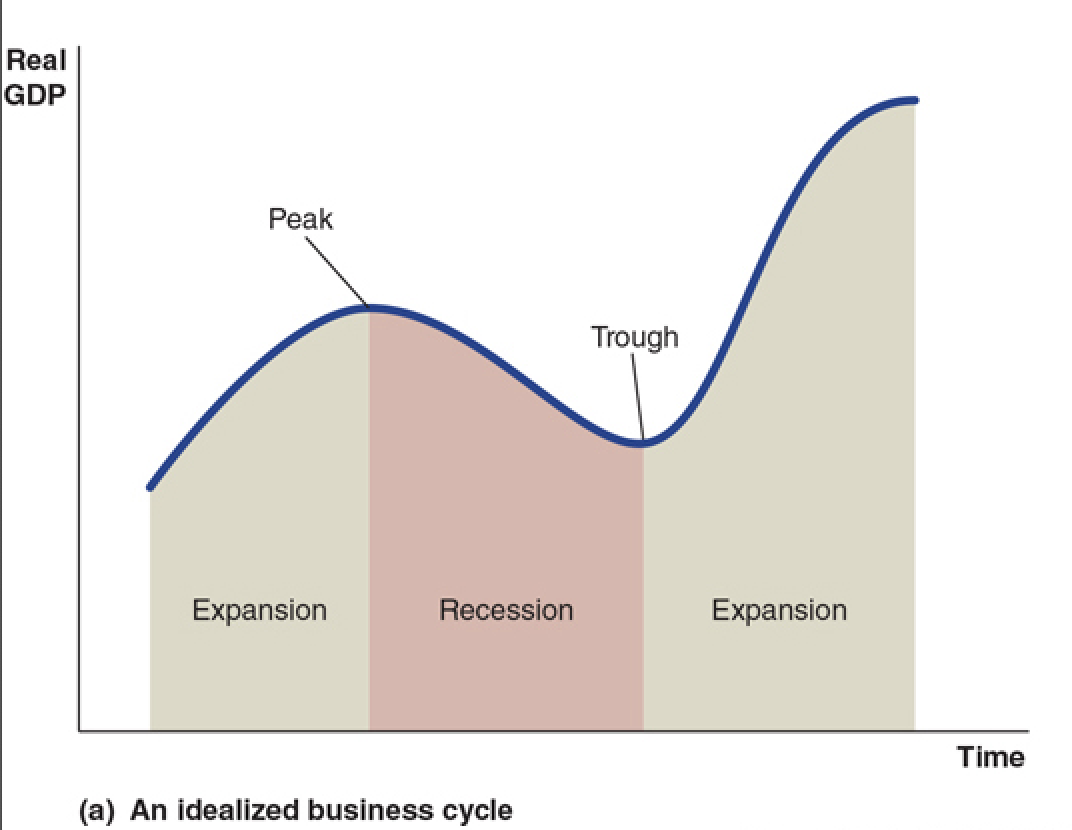
\includegraphics[width=0.61\linewidth]{Fig06-007a}.
\end{frame}

\begin{frame}{Phases of the Business Cycle}
\transfade
\begin{itemize}[<+->]
  \item \textbf{Expansion:} real GDP is rising.
  \item \textbf{Peak:} the point where real GDP stops rising and begins to fall.
  \item \textbf{Recession:} real GDP is falling.
  \item \textbf{Trough:} the point where real GDP stops falling and begins to rise.
  \item After the trough, a new expansion begins.
\end{itemize}
\end{frame}

\begin{frame}{Figure 6.7 -- Canadian Real GDP, 2006--2021 }
\centering
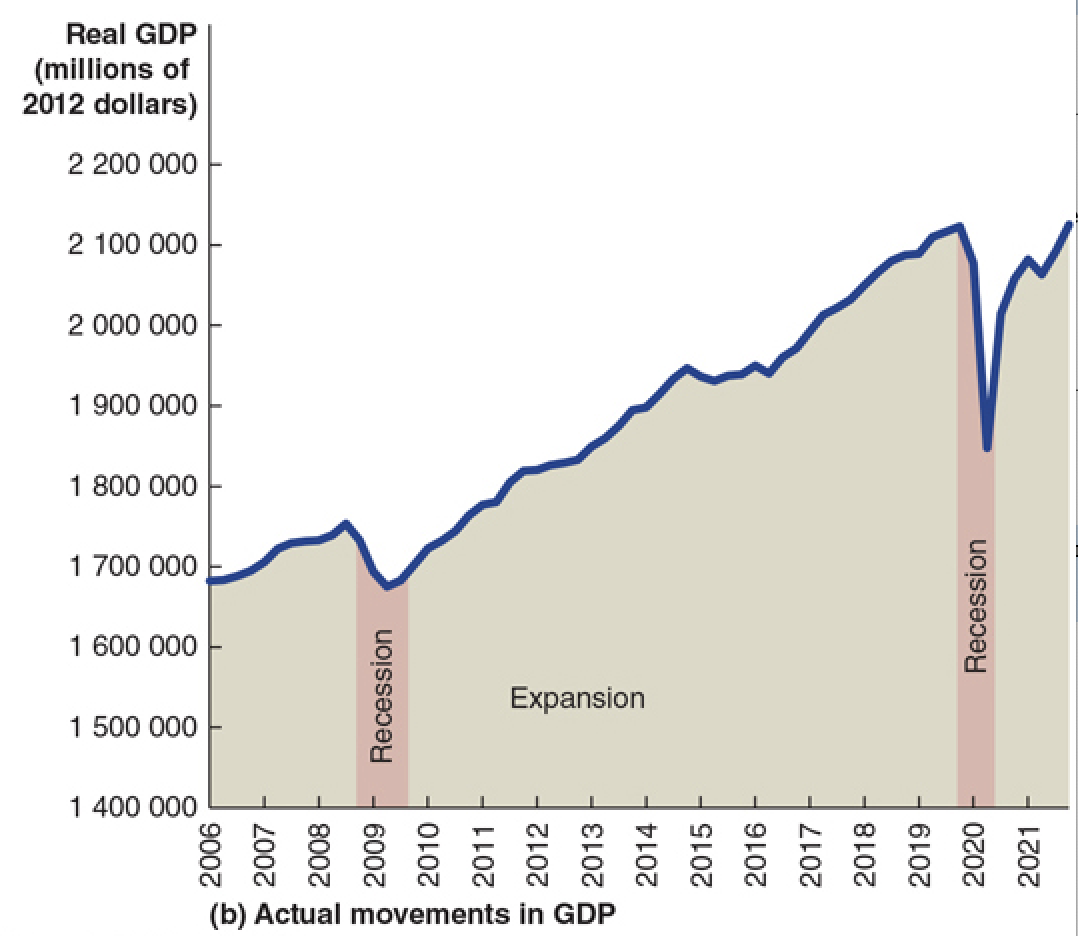
\includegraphics[width=0.561\linewidth]{Fig06-007b}.
\end{frame}

\begin{frame}{Recent Business Cycles in Canada}
\transfade
\begin{itemize}[<+->]
  \item After a peak in 2008:
  \begin{itemize}[<+->]
    \item The economy entered a recession from 2008 to 2009.
    \item Real GDP fell, and unemployment rose.
  \end{itemize}
  \item After the next peak in 2019:
  \begin{itemize}[<+->]
    \item A particularly deep recession occurred during 2020 due to the COVID-19 pandemic.
    \item The trough occurred between April and June 2020.
    \item Real GDP only returned to its 2019 level at the end of 2021.
  \end{itemize}
\end{itemize}
\end{frame}

\begin{frame}{How Do We Know the Economy Is in a Recession?}
\transfade
\begin{itemize}[<+->]
  \item Statistics Canada provides many data series (real GDP, employment, income, etc.).
  \item There is no single Canadian agency that officially declares recessions.
  \item Common rule of thumb:
  \begin{itemize}[<+->]
    \item A recession is two consecutive quarters of negative growth in real GDP.
    \item That is six months of falling real GDP.
  \end{itemize}
\end{itemize}
\end{frame}

% ------------------------------------------------------------
% Business Cycle & Inflation
% ------------------------------------------------------------

\begin{frame}{The Effect of the Business Cycle on Inflation}
\transfade
\begin{itemize}[<+->]
  \item \textbf{Inflation rate:} percentage increase in the price level from one year to the next.
  \item During expansions:
  \begin{itemize}[<+->]
    \item Demand for products is high relative to supply.
    \item Firms can raise prices more easily \(\Rightarrow\) higher inflation.
  \end{itemize}
  \item During recessions:
  \begin{itemize}[<+->]
    \item Demand for products is low relative to supply.
    \item Prices increase more slowly or may even fall \(\Rightarrow\) low inflation or deflation.
  \end{itemize}
\end{itemize}
\end{frame}

\begin{frame}{Figure 6.8 -- Recessions and the Inflation Rate}
\centering
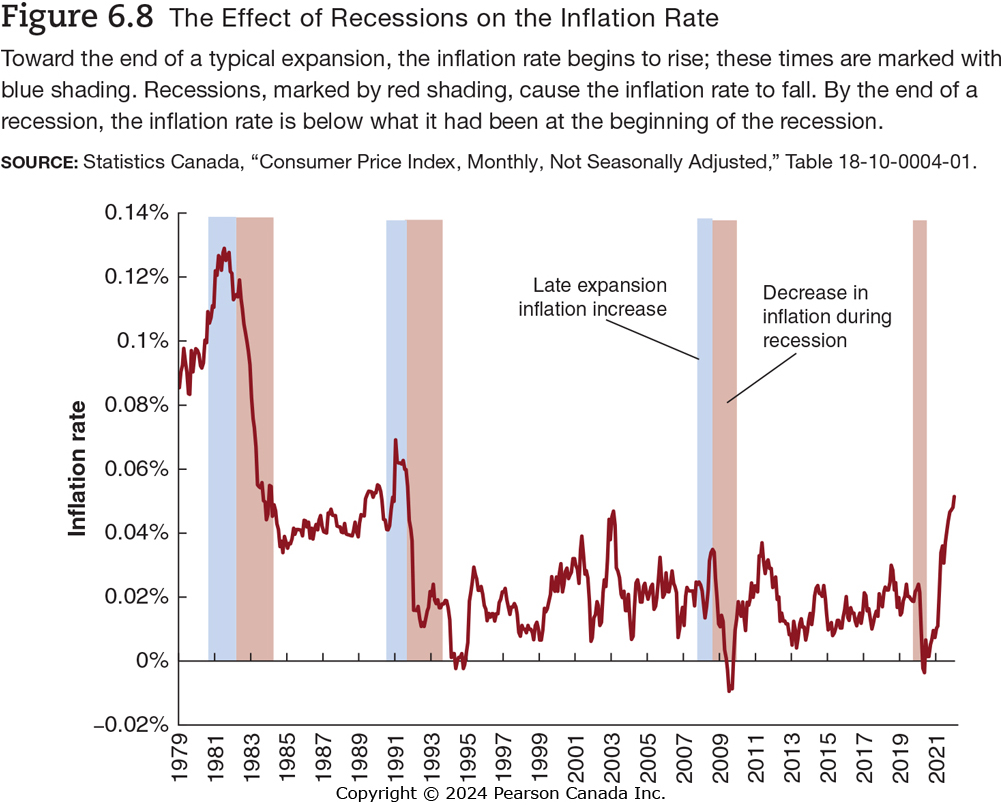
\includegraphics[width=0.71\linewidth]{Fig06-008}.
\end{frame}

\begin{frame}{Inflation Over the Business Cycle}
\transfade
\begin{itemize}[<+->]
  \item In each of the last three Canadian recessions:
  \begin{itemize}[<+->]
    \item Inflation tended to rise during the preceding expansion.
    \item Inflation tended to fall over the course of the recession.
  \end{itemize}
  \item This pattern helps central banks:
  \begin{itemize}[<+->]
    \item use inflation as one indicator of where the economy is in the business cycle.
  \end{itemize}
\end{itemize}
\end{frame}

% ------------------------------------------------------------
% Business Cycle & Unemployment
% ------------------------------------------------------------

\begin{frame}{The Effect of the Business Cycle on Unemployment}
\transfade
\begin{itemize}[<+->]
  \item During recessions:
  \begin{itemize}[<+->]
    \item Firms see sales fall.
    \item They reduce production.
    \item They lay off workers.
  \end{itemize}
  \item \textbf{Unemployment} often continues to rise even after a recession begins.
  \item During expansions:
  \begin{itemize}[<+->]
    \item Firms hire more workers.
    \item Unemployment gradually falls.
  \end{itemize}
\end{itemize}
\end{frame}

\begin{frame}{Figure 6.9 -- Recessions and the Unemployment Rate}
\centering
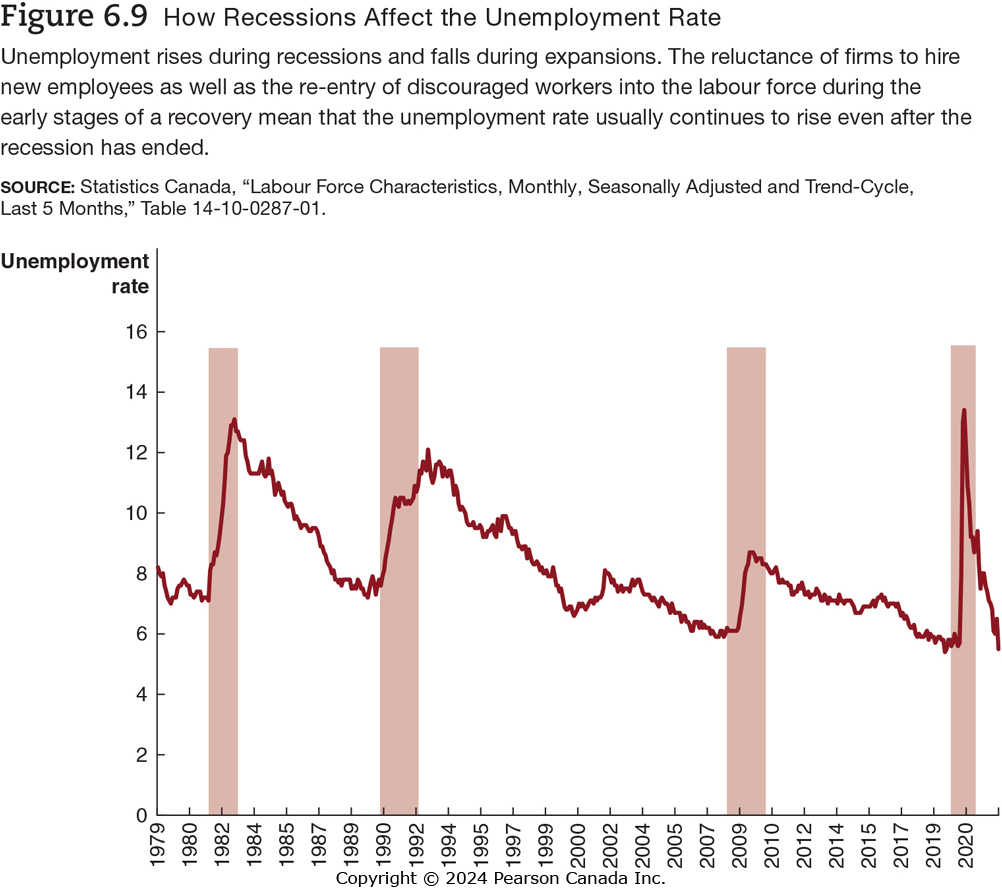
\includegraphics[width=0.71\linewidth]{Fig06-009}.
\end{frame}

\begin{frame}{Putting It All Together}
\transfade
\begin{itemize}[<+->]
  \item \textbf{Long-run trend:}
  \begin{itemize}[<+->]
    \item Real GDP per capita grows as productivity rises.
  \end{itemize}
  \item \textbf{Short-run fluctuations:}
  \begin{itemize}[<+->]
    \item Business cycles around the trend.
    \item Recessions associated with:
    \begin{itemize}[<+->]
      \item lower output,
      \item lower inflation,
      \item higher unemployment.
    \end{itemize}
  \end{itemize}
  \item \textbf{Financial system:}
  \begin{itemize}[<+->]
    \item Channels saving into investment, supporting long-run growth.
    \item Government borrowing can crowd out some private investment.
  \end{itemize}
\end{itemize}
\end{frame}

% ============================================================
\section*{Chapter Summary}
% ============================================================

\begin{frame}{Summary}
\transfade
\begin{itemize}[<+->]
  \item Long-run economic growth is driven by \textbf{labour productivity}, which depends on:
  \begin{itemize}[<+->]
    \item capital per worker,
    \item human capital,
    \item technological change.
  \end{itemize}
  \item Potential GDP and the \textbf{output gap} help us see whether resources are over- or under-utilized.
  \item The \textbf{financial system} provides:
  \begin{itemize}[<+->]
    \item risk-sharing,
    \item liquidity,
    \item information.
  \end{itemize}
  \item In a closed economy, \textbf{saving equals investment}:
  \begin{itemize}[<+->]
    \item budget deficits can crowd out private investment.
  \end{itemize}
  \item The \textbf{business cycle} describes short-run fluctuations in real GDP, with:
  \begin{itemize}[<+->]
    \item expansions, peaks, recessions, and troughs,
    \item characteristic movements in inflation and unemployment.
  \end{itemize}
\end{itemize}
\end{frame}

\begin{frame}
\centering
\Huge \textbf{Thank you!}
\end{frame}

\end{document}
